\begin{frame}{\expvi}
	\textbf{motivation:}
	\begin{itemize}
		\item we observed problems for computed correlations for both character and word level
		\item how can we still obtain the neurons showing \textit{consistency} in their behaviour (even if not over all sequences)
		\item we could plot all sentence activations and count, but well ...
		\item how can we figure out groups of neurons, that “work together“
	\end{itemize}
\end{frame}
\begin{frame}{\expvi}
	\textbf{procedure:}
	\begin{itemize}
		\item take correlation values from E5 and find $k$ strongest neurons for each sentence ($k=100$ out of 512 per layer $\times$ (cells, states))
		\item memorize these neurons for each layer
		\item cluster the sentences (which sentences have the most in common)
		\item plot some sentences to get an idea what these correlation values are about 
	\end{itemize}
\end{frame}
\begin{frame}{\expvi}
	\textbf{results:}
	\begin{itemize}
		\item the intersection of top $k$ neurons over all sentences was \textbf{empty}
		\item but \dots
	\end{itemize}
\end{frame}
\begin{frame}{\expvi}
	\begin{figure}
		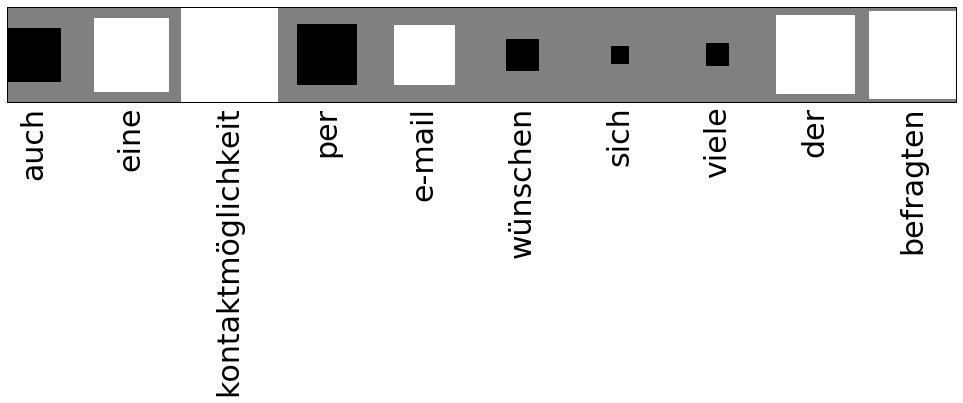
\includegraphics[width=200pt,height=100pt]{gfx/perfectneuron.png}
		\caption{LSTM, first hidden layer cells output (neuron 36)} % consitent over time
	\end{figure}
\end{frame}
\begin{frame}{\expvi}
	\begin{figure}
		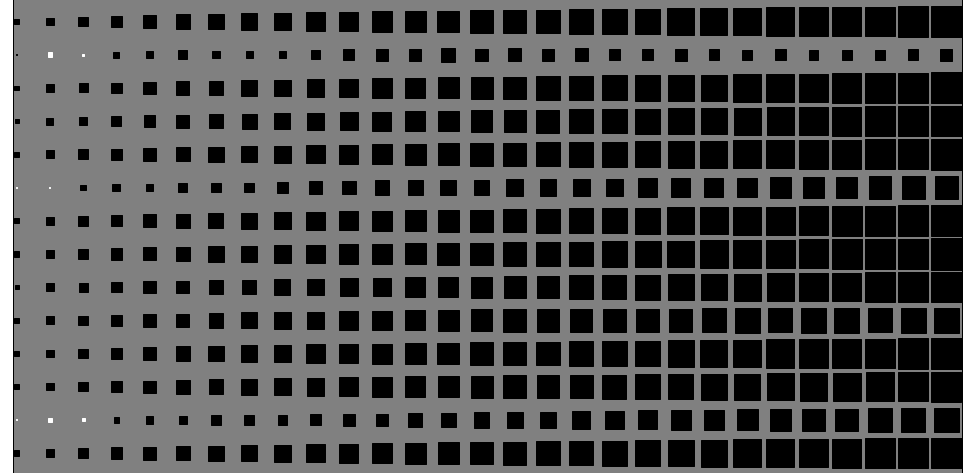
\includegraphics[width=200pt,height=100pt]{gfx/cells1length.png}
		\caption{LSTM, last hidden layer cells output (observed way more often)} % consitent over time
	\end{figure}
\end{frame}
\begin{frame}{\expvi}
	\textbf{conclusion:}
	\begin{itemize}
		\item a combined method of plotting and correlating only provided a clear answer (so far), both methods on its own seem to be insufficient
		\item indeed the computed correlations seem to have been mostly about sentence length
		\item no neuron (in the inspected areas) showed strong correlations over all sentences
		\item neurons seem to act in clusters, but these are also not constant over time
		\item there are no hints or observations, that the network captured the hierarchical relation, but somehow distributional properties of nouns with their determiners	
	\end{itemize}
\end{frame}